\documentclass[11pt,a4paper]{report}
\usepackage[portuges]{babel}
\usepackage[utf8]{inputenc} 
\usepackage{graphicx} 
\usepackage{url} 
\usepackage{enumerate} 
\usepackage{color} 
\usepackage{textcomp}
\usepackage{indentfirst}
\usepackage{array} 
\usepackage{parskip}
\usepackage[export]{adjustbox}
\usepackage{xpatch}
\usepackage{amsmath}
\newlength{\chaptertopskip}
\setlength{\chaptertopskip}{10pt}

\usepackage{a4wide}
\usepackage{float}
\usepackage{minted}
\usepackage{multicol}
\usepackage{appendix}
\setlength{\parskip}{1em}
\usepackage{verbatim}

\usepackage[demo]{graphicx}
\usepackage{caption}
\usepackage{subcaption}


\usepackage[pdftex]{hyperref} % transformar as referências internas do seu documento em hiper-ligações.

\definecolor{saddlebrown}{rgb}{0.55, 0.27, 0.07} % para definir uma nova cor, neste caso 'saddlebrown'

\usepackage{listings}  % para utilizar blocos de texto verbatim no estilo 'listings'
%paramerização mais vulgar dos blocos LISTING - GENERAL
\lstset{
	basicstyle=\small, %o tamanho das fontes que são usadas para o código
	numbers=left, % onde colocar a numeração da linha
	numberstyle=\tiny, %o tamanho das fontes que são usadas para a numeração da linha
	numbersep=5pt, %distancia entre a numeração da linha e o codigo
	breaklines=true, %define quebra automática de linha
    frame=tB,  % caixa a volta do codigo
	mathescape=true, %habilita o modo matemático
	escapeinside={(*@}{@*)} % se escrever isto  aceita tudo o que esta dentro das marcas e nao altera
}

\usepackage{xspace} % deteta se a seguir a palavra tem uma palavra ou um sinal de pontuaçao se tiver uma palavra da espaço, se for um sinal de pontuaçao nao da espaço

\parindent=20pt %espaço a deixar para fazer a  indentação da primeira linha após um parágrafo
\parskip=10pt % espaço entre o parágrafo e o texto anterior

\setlength{\oddsidemargin}{-1cm} %espaço entre o texto e a margem
\setlength{\textwidth}{18cm} %Comprimento do texto na pagina
\setlength{\headsep}{0cm} %espaço entre o texto e o cabeçalho
\setlength{\textheight}{23cm} %altura do texto na pagina
\renewcommand{\baselinestretch}{1.5cm}


\begin{document}
\begin{figure}
    
\includegraphics[scale=0.3]{logoum.png}
\end{figure}
\title{\textbf{Normais e Coordenadas de Texturas}\\
       \textbf{Unidade Curricular de Computação Gráfica}\\ Licenciatura em Ciências da Computação\\Universidade do Minho
       } %Titulo do documento
\author{Bruno Jardim\\ (A91680) \and Inês Presa\\ (A90355)
         \and Tiago Carriço\\ (A91695) \and Tiago Leite\\ (A91693)
       } %autores do documento
\date{\today} %data
\maketitle
\begingroup
\renewcommand*\contentsname{Índice}
\let\clearpage\relax
\tableofcontents


\endgroup
\newpage

\chapter{Contextualização}    
No âmbito da unidade curricular de Computação Gráfica da Licenciatura em Ciências da Computação foi proposto o desenvolvimento em \textit{Opengl} de um motor gráfico genérico que terá como função a criação de um sistema solar. Desenvolvimento esse que deve ser composto por quatro etapas. 

\section{Enunciado}
Nesta quarta etapa foi proposto:

\begin{itemize}
    \item \textbf{Normais e coordenadas de texturas dos modelos}
        \begin{description}
        \item Alteração do \textit{generator} para produzir as normais dos modelos gerados. 
        \item Alteração do \textit{generator} para produzir as cordenadas de textura dos modelos gerados.
        \end{description}
        
    \item \textbf{Iluminação}
        \begin{description}
        \item Alteração do \textit{engine} para aplicar a iluminação definida no ficheiro de configuração \textit{xml}. 
        \end{description}
    \item \textbf{Texturas}
        \begin{description}
        \item Alteração do \textit{engine} para aplicar as texturas definidas no ficheiro de configuração \textit{xml}. 
        \end{description}

    \item \textbf{Sistema solar com iluminação e texturas}
    \begin{description}
    \item Alteração do ficheiro de configuração \textit{xml} de modo a gerar um modelo do sistema solar com iluminação e texturas.
    \end{description}

\end{itemize}


\chapter{Apresentação das soluções}
\section{Normais e coordenadas de texturas dos modelos}

\subsection{Plano}
As normais do plano são (0,1,0) para todos os seus pontos.\\

As coordenadas de textura do plano são calculadas de acordo com a variação de $x$ e $z$ nos dois ciclos de geração dos vértices.Ou seja, se o plano tiver $d$ divisões, as coordenadas do vértice $(x,0,z)$ serão associadas ás coordenadas de textura $(x/d ,y/d)$.

\subsection{Cubo}
As normais do cubo são as seguintes:
\begin{itemize}
    \item Topo : (0,1,0)
    \item Base : (0,-1,0)
    \item Frente : (0,0,1)
    \item Trás : (0,0,-1)
    \item Direita : (1,0,0)
    \item Esquerda : (-1,0,0)
\end{itemize}

Para o cálculo das coordenadas de textura do cubo, foi utilizada a mesma estratégia do plano para cada uma das suas faces.

\subsection{Esfera}
As normais, $n$, da esfera são calculadas com as coordenadas polares dos vértices sem o uso do valor do raio, da seguinte forma:
\begin{itemize}
    \item $x = cos(\beta)*sin(\alpha)$
    \item $y = sin(\beta)$
    \item $z = cos(\beta)*cos(\alpha)$
    \item $n = (x, y, z)$ 
\end{itemize}

Sendo que, o $\beta$ varia entre $-90 \text{\textdegree} $ e $90 \text{\textdegree}$ e o $\alpha$ varia entre $0 \text{\textdegree}$ e $360 \text{\textdegree}$.

As coordenadas de textura da esfera são calculadas utilizando as variáveis de iteração $(i, j)$ nos dois ciclos de cálculo dos valores dos vértices de cada triângulo da esfera. Por exemplo, se $i$ iterar pelas \textit{slices} e $j$ iterar pelas \textit{stacks}, as coordenadas de textura do vértice $P$ serão constituídas pelos seguintes pontos:
\begin{itemize}
    \item $x = raio*cos(90 \text{\textdegree} - \beta'*j)*sin(\alpha'*i)$
    \item $y = raio*sin(90 \text{\textdegree} - \beta'*j)$
    \item $z = raio*cos(90 \text{\textdegree} - \beta'*j)*cos(\alpha'*i)$
\end{itemize}
Com $\alpha' =  360 \text{\textdegree}/slices$ e $\beta' =  180 \text{\textdegree}/stacks$.

As coordenadas de texturas de $P$ serão $(i/slices, j/stacks)$. 

\subsection{Cone}
Para o cone, à semelhança do que acontece com o calculo dos vértices de cada triângulo, o processo de cálculo das normais e coordenadas de textura foi dividido em base e corpo.

Para a base as normais são $(0,-1,0)$ para todos os seus pontos. Para as coordenadas de textura, o ponto central tem as coordenadas $(0.5,0.5)$ e os restantes são calculados com os valores das coordenadas de cada vértice sem o uso do valor do raio da seguinte forma:
\begin{itemize}
    \item $x = 0.5 + sin(\alpha)$
    \item $y = 0$
    \item $z = 0.5 + cos(\alpha)$
\end{itemize}
Com $\alpha$  a variar entre $0 \text{\textdegree}$ e $360 \text{\textdegree}$.

Para o corpo do cone, se se considerar $i$ como a variável que itera pelo número de \textit{stacks} e $j$ como a variável que itera pelo número de \textit{slices} e que cada ponto $P$ tem as seguintes coordenadas:
\begin{itemize}
    \item $x = r*sin(\alpha*j)$
    \item $y = i*stack\_size$
    \item $z = r*cos(\alpha*j)$
\end{itemize}
Com:
\begin{itemize}
    \item $stack\_size =  height/stacks$
    \item $\alpha = 360 \text{\textdegree}/slices$
    \item $r = (height - i*stack\_size)/(height/radius)$
\end{itemize} 
As normais de $P$ têm os valores $(x,y,z)$, com:
\begin{itemize}
    \item $x = sin(\alpha*j)$
    \item $y = sin(atan(radius/height)$
    \item $z = cos(\alpha*j)$
\end{itemize}

As coordenadas de textura de $P$ são $(j/slices, i/stacks)$

\subsection{Cilindro}

O cálculo das normais e coordenadas de textura do cilindro foi divido em base, topo e corpo.

Para a a base e topo utilizou-se a mesma estratégia da base do cone, com as devidas adaptações no topo, pois esta face encontra-se virada para direção oposta.

Para o corpo do cilindro, para cada ponto, os valores das normais em $x$ e $z% são calculados com a mesma estratégia do corpo do cone e o valor de $y$ é sempre 0.

O cálculo das coordenadas de textura no corpo do cilindro é feito com a mesma estratégia do corpo do cone.


\subsection{Torus}

Seja $P$ um ponto do torus em que as suas coordenadas são calculadas da seguinte forma:

\begin{itemize}
    \item $x = (R + r*cos(\alpha*i))*cos(\beta*j)$
    \item $y = r*sin(\alpha*i)$
    \item $z = (R + r*cos(\alpha*i))*sin(\beta*j)$
\end{itemize}
Com:
\begin{itemize}
    \item $i$  a variável que itera pelo número de \textit{stacks}
    \item $j$  a variável que itera pelo número de \textit{slices}
    \item $\alpha = 360 \text{\textdegree}/stacks$
    \item $\beta = 360 \text{\textdegree}/slices$
    \item $R = (raio+espessura)/2$
    \item $r = R - espessura$
\end{itemize} 
As normais de $P$ têm os valores $(x,y,z)$, com:
\begin{itemize}
    \item $x = r*cos(\alpha*i)*cos(\beta*j)$
    \item $y = r*sin(\alpha*i)$
    \item $z = r*cos(\alpha*i)*sin(\beta*j)$
\end{itemize}

As coordenadas de textura de $P$ são $(i/stacks, j/slices)$

\subsection{Bezier}
Relembrando que para o processo de cálculo dos pontos necessários à construção de cada superfície foi utilizada a seguinte fórmula:
\par
Seja a matriz de Bezier \emph{M =}
\begin{bmatrix}
-1 & 3 & -3 & 1\\
3 & -6 & 3 & 0\\
-3 & 3 & 0 & 0\\
1 & 0 & 0 & 0
\end{bmatrix}
\par
\emph{T =} nível de tesselação
\par
4 curvas de Bezier \emph{$C_0$,$C_1$,$C_2$,$C_3$}
\par
\emph{$C_0 = P_{00} , P_{10} , P_{20} , P_{30}$}
\par
\emph{$C_1 = P_{01} , P_{11} , P_{21} , P_{31}$}
\par
\emph{$C_2 = P_{02} , P_{12} , P_{22} , P_{32}$}
\par
\emph{$C_3 = P_{03} , P_{13} , P_{23} , P_{33}$}
\par
\emph{$B(u,v) =$}
\begin{bmatrix}
\emph{$u^3$} & \emph{$u^2$} & \emph{$u$} & \emph{$1$}\\
\end{bmatrix}
\emph{$M$}
\begin{bmatrix}
\emph{$P_{00}$} & \emph{$P_{01}$} & \emph{$P_{02}$} & \emph{$P_{03}$}\\
\emph{$P_{10}$} & \emph{$P_{11}$} & \emph{$P_{12}$} & \emph{$P_{13}$}\\
\emph{$P_{20}$} & \emph{$P_{21}$} & \emph{$P_{22}$} & \emph{$P_{23}$}\\
\emph{$P_{30}$} & \emph{$P_{31}$} & \emph{$P_{32}$} & \emph{$P_{33}$}
\end{bmatrix} 
\emph{$M^T$}
\begin{bmatrix}
\emph{$v^3$}\\
\emph{$v^2$}\\
\emph{$v$} \\
\emph{$1$} 
\end{bmatrix}
\par
Os vários pontos da superfície são obtidos utilizando a função \emph{B} variando \emph{u} e \emph{v} entre 0 e 1.
\par
Por exemplo com:
\par
\emph{a = B(0,0) b = B(1/T,0) c = B(1/T,1/T) d = B(0,1/T)}
\par
Podem-se construir os triângulos \emph{a,b,d} e \emph{b,c,d}.

Para calcular as normais de um ponto calcula-se: 

\emph{$u'=$}
\begin{bmatrix}
\emph{$3*u^2$} & \emph{$2*u$} & \emph{$1$} & \emph{$0$}\\
\end{bmatrix}
\emph{$M$}
\begin{bmatrix}
\emph{$P_{00}$} & \emph{$P_{01}$} & \emph{$P_{02}$} & \emph{$P_{03}$}\\
\emph{$P_{10}$} & \emph{$P_{11}$} & \emph{$P_{12}$} & \emph{$P_{13}$}\\
\emph{$P_{20}$} & \emph{$P_{21}$} & \emph{$P_{22}$} & \emph{$P_{23}$}\\
\emph{$P_{30}$} & \emph{$P_{31}$} & \emph{$P_{32}$} & \emph{$P_{33}$}
\end{bmatrix} 
\emph{$M^T$}
\begin{bmatrix}
\emph{$v^3$}\\
\emph{$v^2$}\\
\emph{$v$} \\
\emph{$1$} 
\end{bmatrix}
\par

\emph{$v'=$}
\begin{bmatrix}
\emph{$u^3$} & \emph{$u^2$} & \emph{$u$} & \emph{$1$}\\
\end{bmatrix}
\emph{$M$}
\begin{bmatrix}
\emph{$P_{00}$} & \emph{$P_{01}$} & \emph{$P_{02}$} & \emph{$P_{03}$}\\
\emph{$P_{10}$} & \emph{$P_{11}$} & \emph{$P_{12}$} & \emph{$P_{13}$}\\
\emph{$P_{20}$} & \emph{$P_{21}$} & \emph{$P_{22}$} & \emph{$P_{23}$}\\
\emph{$P_{30}$} & \emph{$P_{31}$} & \emph{$P_{32}$} & \emph{$P_{33}$}
\end{bmatrix} 
\emph{$M^T$}
\begin{bmatrix}
\emph{$3*v^2$}\\
\emph{$2*v$}\\
\emph{$1$} \\
\emph{$0$} 
\end{bmatrix}
\par

Cada normal de cada componente de $P$ é obtida fazendo $u'\times v'/||u'\times v'||$.

As coordenadas de textura de $P$ são simplesmente (v,u).
\newpage

\section{Iluminação}

Para a iluminação da cena criou-se duas classes \textit{abstracts}. A classe \textit{Light} e a classe \textit{Color}.

A classe \textit{Light} é estendida pelas classes:

\begin{itemize}
    \item \textit{LightPoint}
    \item \textit{LightDirectional}
    \item \textit{LightSpotlight} 
\end{itemize}
\newline

A classe Color é \textit{estendida} pelas classes:

\begin{itemize}
    \item \textit{Diffuse}
    \item \textit{Ambient}
    \item \textit{Specular}
    \item \textit{Emissive}
    \item \textit{Shininess}
\end{itemize}

Na leitura do ficheiro \textit{xml}, caso este possua informação de iluminação, controi-se instâncias da classe \textit{Light}, de acordo com o tipo de luz, e armazena-se estas num vetor. Na função \textit{renderScence} este vetor vai é percorrido e cada uma das "luzes" armazenadas será aplicada. 
Cada \textit{model} possui agora também um vetor de \textit{Color} onde se aramazena as propriedades de iluminação dos seus materiais e a informação do \textit{VBO} onde estão guardadas as normais de cada ponto. No momento em que os \textit{models} são desenhados, o vetor de \textit{Color} é percorrido e as propriedades dos materiais são aplicadas.
\par
Nesta fase, tal como na anterior criou-se um \textit{map} de primitivas para vetor de normais e um \textit{map} de primitivas para \textit{VBO} das normais, de forma a que para cada primitiva as suas normais apenas sejam lidas as normais uma vez e apenas exista um \textit{VBO} onde estas ficam guardadas. 
\subsection{Demonstração}

\begin{figure}[H]
\centering
\begin{subfigure}{0.5\textwidth}
  \centering
  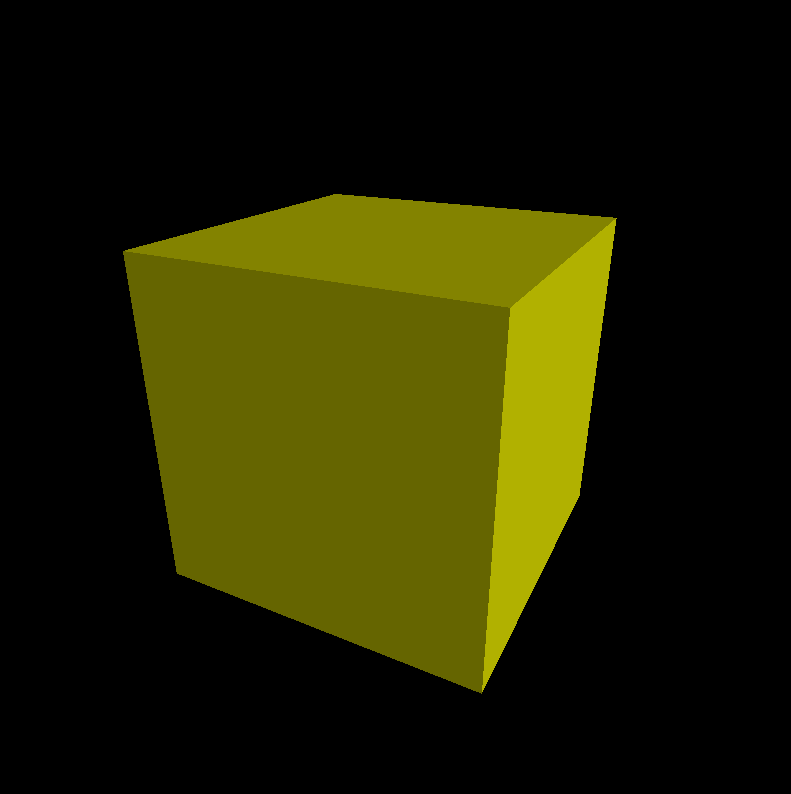
\includegraphics[width = 8cm,height = 8cm]{test_4_1.png}
  \caption{\texttt{test\_4\_1.xml}}
  \label{fig:test_4_1}
\end{subfigure}%
\begin{subfigure}{0.5\textwidth}
  \centering
  
\includegraphics[width = 8cm,height = 8cm]{test_4_2.png}
  \caption{\texttt{test\_4\_2.xml}}
  \label{fig:test_4_2}
\end{subfigure}
\begin{subfigure}{0.5\textwidth}
  \centering
  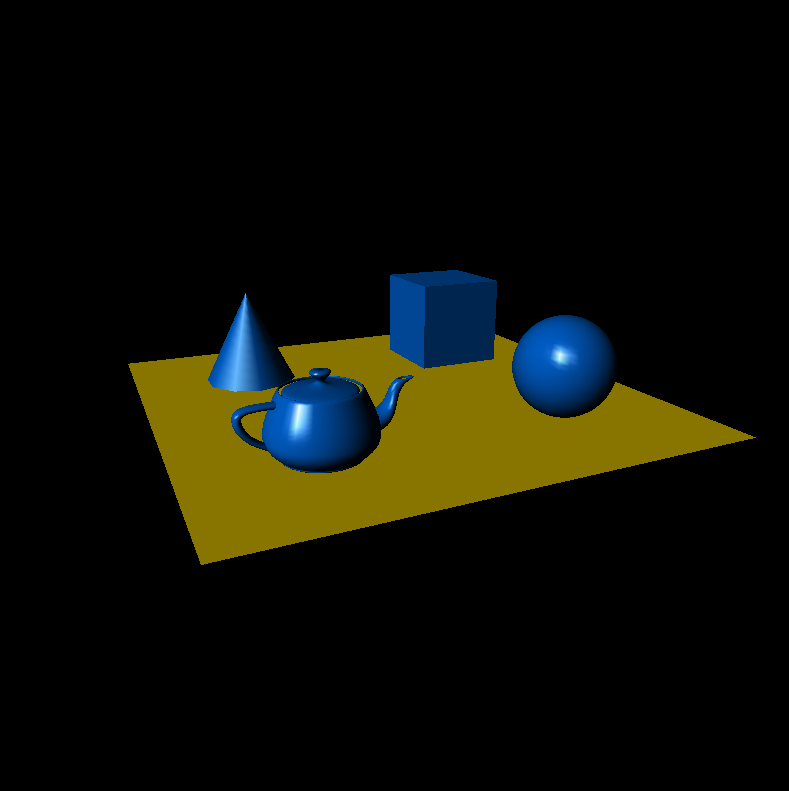
\includegraphics[width = 8cm,height = 8cm]{test_4_3.png}
  \caption{\texttt{test\_4\_3.xml}}
  \label{fig:test_4_3}
\end{subfigure}%
\begin{subfigure}{0.5\textwidth}
  \centering
  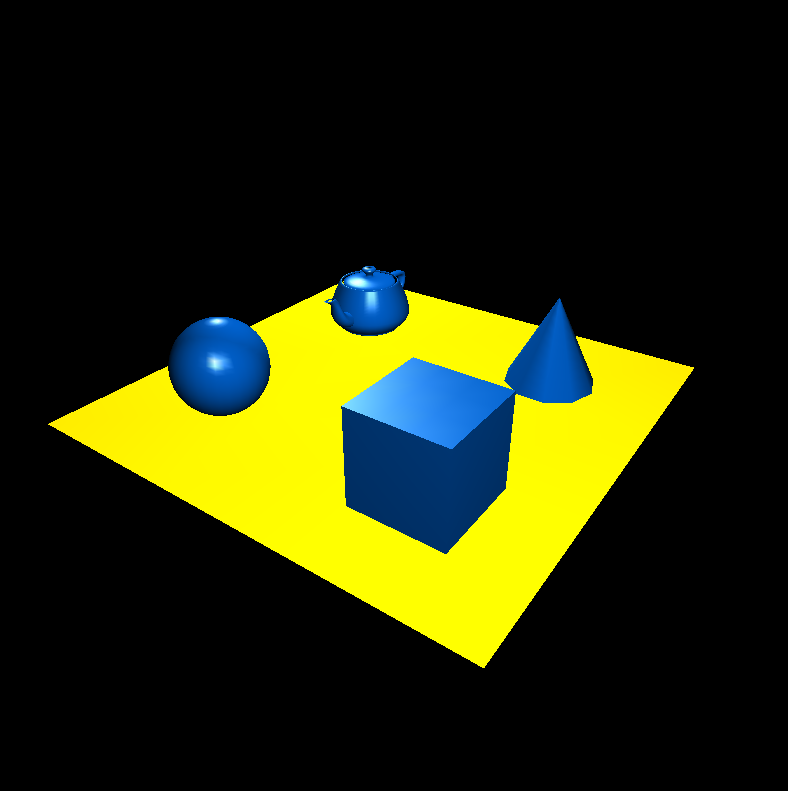
\includegraphics[width = 8cm,height = 8cm]{test_4_4.png}
  \caption{\texttt{test\_4\_4.xml}}
  \label{fig:test_4_4}
\end{subfigure}
\end{figure}
\newpage
\begin{figure}[H]
\centering
\begin{subfigure}{0.5\textwidth}
  \centering
  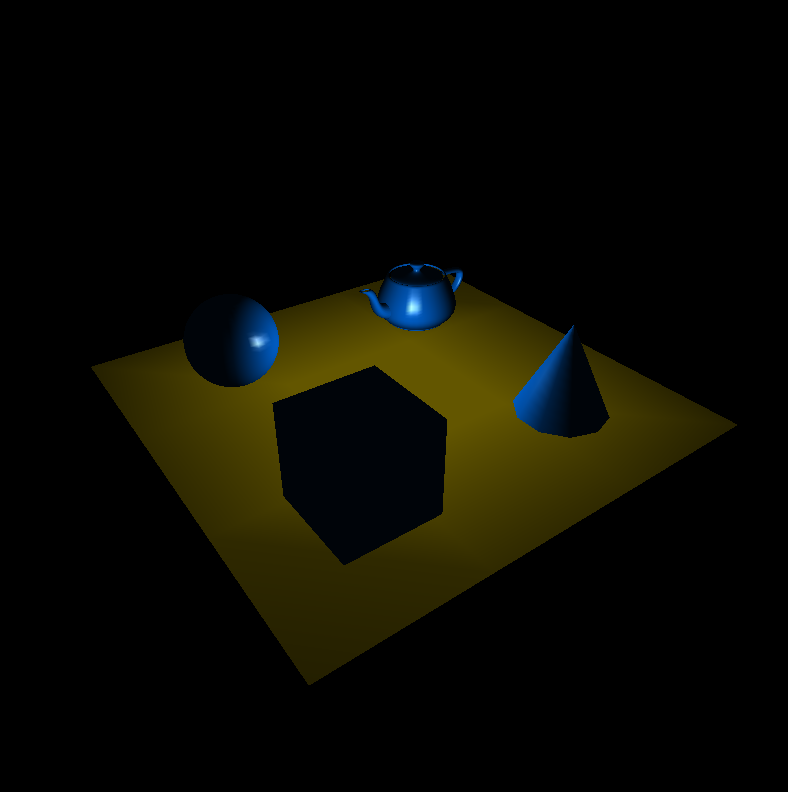
\includegraphics[width = 8cm,height = 8cm]{test_4_5.png}
  \caption{\texttt{test\_4\_5.xml}}
  \label{fig:test_4_5}
\end{subfigure}%
\begin{subfigure}{0.5\textwidth}
  \centering
  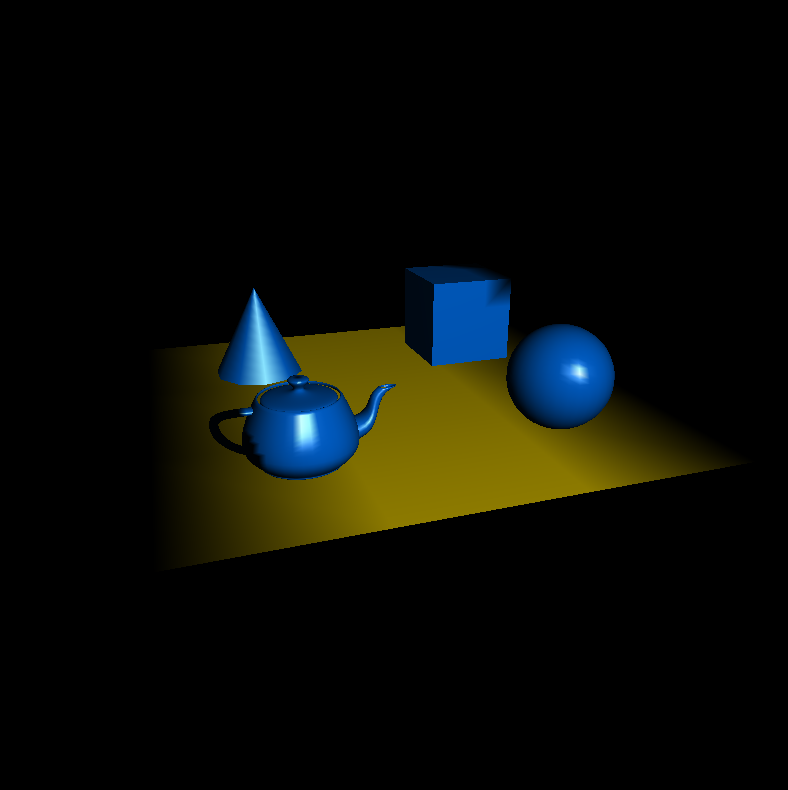
\includegraphics[width = 8cm,height = 8cm]{test_4_6.png}
  \caption{\texttt{test\_4\_6.xml}}
  \label{fig:test_4_6}
\end{subfigure}
\begin{subfigure}{0.5\textwidth}
  \centering
  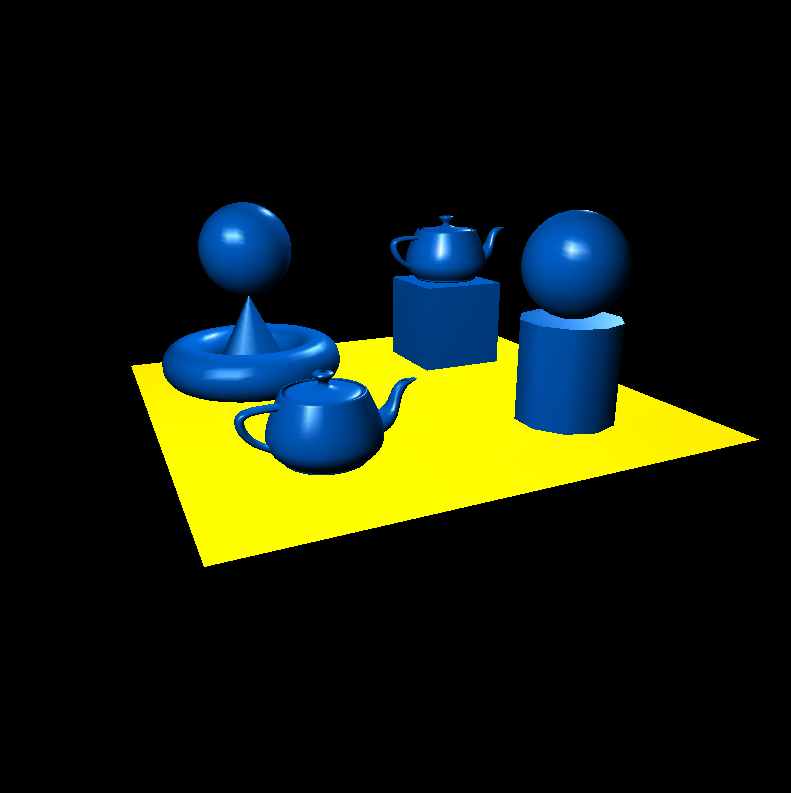
\includegraphics[width = 8cm,height = 8cm]{test_light.png}
  \caption{\texttt{test\_light.xml}}
  \label{fig:test_light}
\end{subfigure}%
\begin{subfigure}{0.5\textwidth}
  \centering
  
\includegraphics[width = 8cm,height = 8cm]{snowman.png}
  \caption{\texttt{snowman.xml}}
  \label{fig:snowman}
\end{subfigure}
\caption{Iluminação}
\end{figure}

\newpage
\section{Texturas}
Para as texturas, foi adicionou-se para cada \textit{model} uma variável a indicar qual o \textit{VBO} com as coordenadas de textura e outra com a informação gerada pela função \textit{glGenTextures}.

O \textit{engine} analisa o ficheiro de configuração de \textit{xml} e caso os modelos possuam texturas as suas coordenadas são lidas e armazenadas num vetor de coordenadas de textura, cada textura é carregada e a sua informação é armazenada junto do \textit{model} respetivo.
Tal como nas coordenadas de posição e na iluminação, aqui também se utiliza um \textit{map} de primitivas para o vetor de coordenadas de textura e um mapa de apontadores de textura para a textura. Assim, cada textura é lida apenas uma vez e cada primitiva apenas vai possuir um \textit{VBO} com as suas coordenadas de textura.

\subsection{Demonstração}

\vspace{1cm}
\begin{figure}[H]
\centering
\begin{subfigure}{0.5\textwidth}
  \centering
  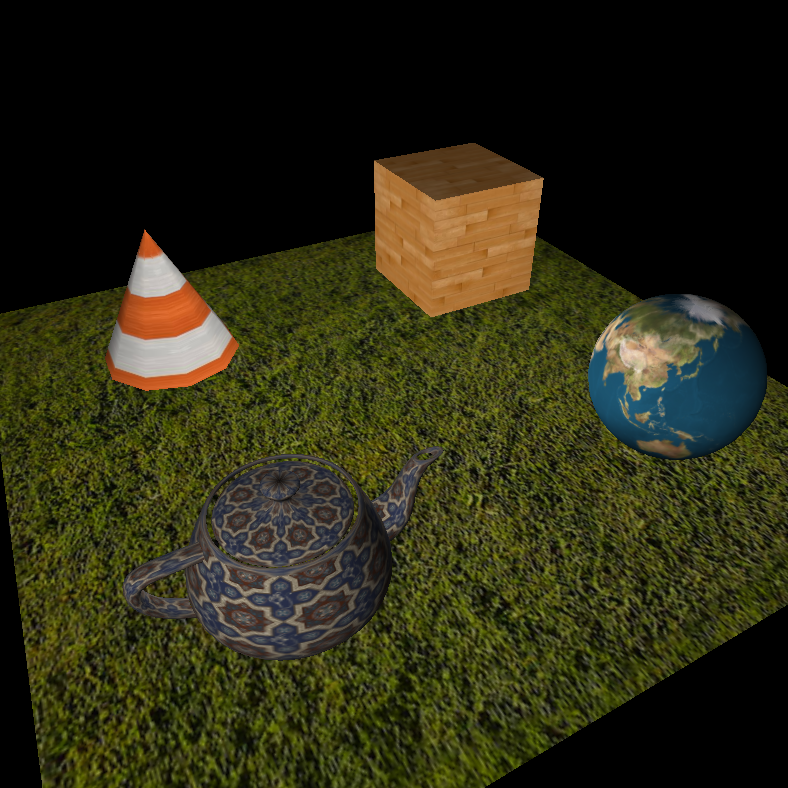
\includegraphics[width = 8cm,height = 8cm]{test_4_7.png}
  \caption{\texttt{}}
  \label{fig:test_4_7}
\end{subfigure}%
\begin{subfigure}{0.5\textwidth}
  \centering
  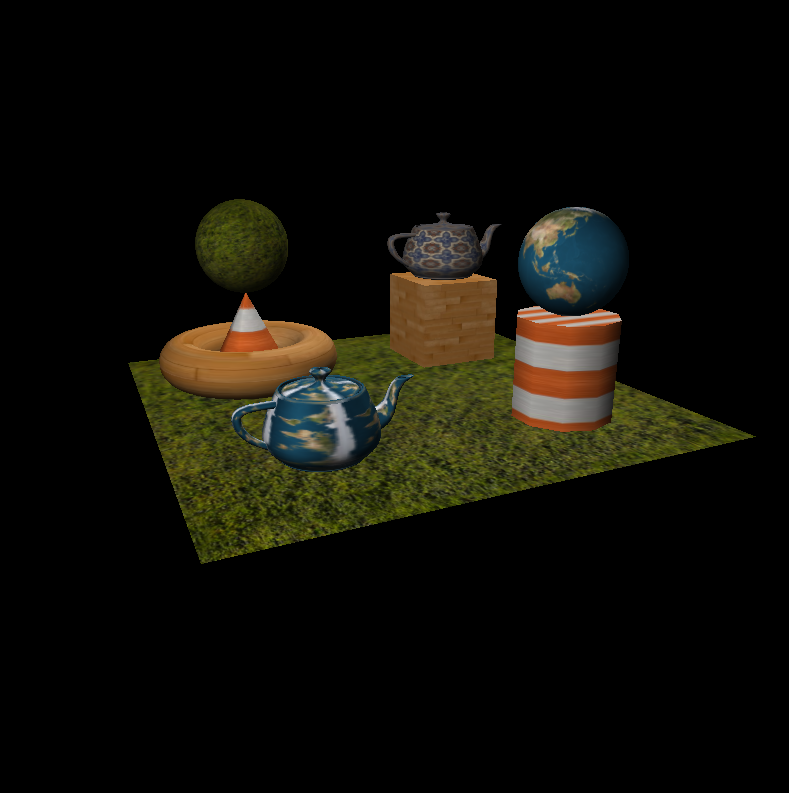
\includegraphics[width = 8cm,height = 8cm]{test_tex.png}
  \caption{\texttt{}}
  \label{fig:test_tex}
\end{subfigure}
\label{fig:texturas}
\caption{Texturas}
\end{figure}

\newpage
\section{Sistema solar com iluminação e texturas}

Para iluminar o sistema solar colocou-se um ponto de luz no ponto (0,0,0) e definiu-se o sol como um objeto emissivo.
Colocou-se texturas a todos os objetos do sistema solar.

\subsection{Demonstração}
\vspace{1cm}
\begin{figure}[H]
\centering
\begin{subfigure}{0.5\textwidth}
  \centering
  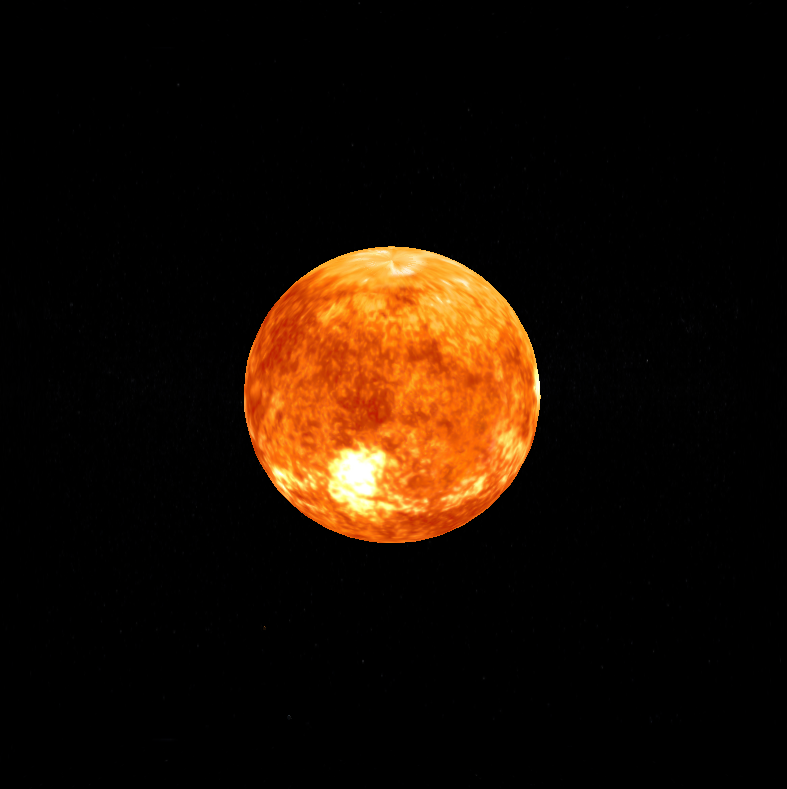
\includegraphics[width = 8cm,height = 8cm]{sun.png}
  \caption{\texttt{}}
  \label{fig:sun}
\end{subfigure}%
\begin{subfigure}{0.5\textwidth}
  \centering
  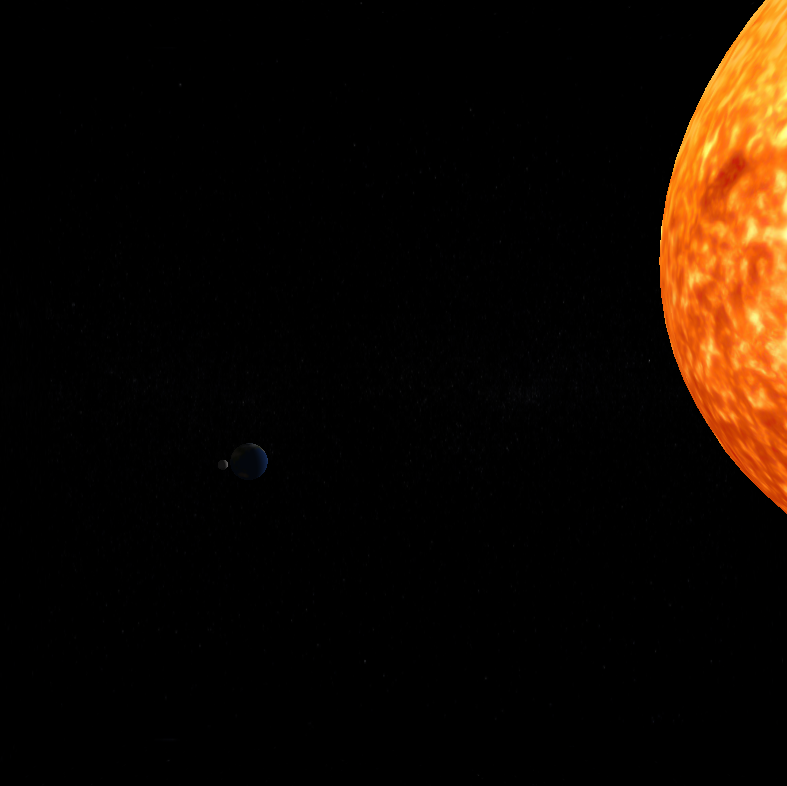
\includegraphics[width = 8cm,height = 8cm]{earth.png}
  \caption{\texttt{}}
  \label{fig:earth}
\end{subfigure}
\begin{subfigure}{0.5\textwidth}
  \centering
  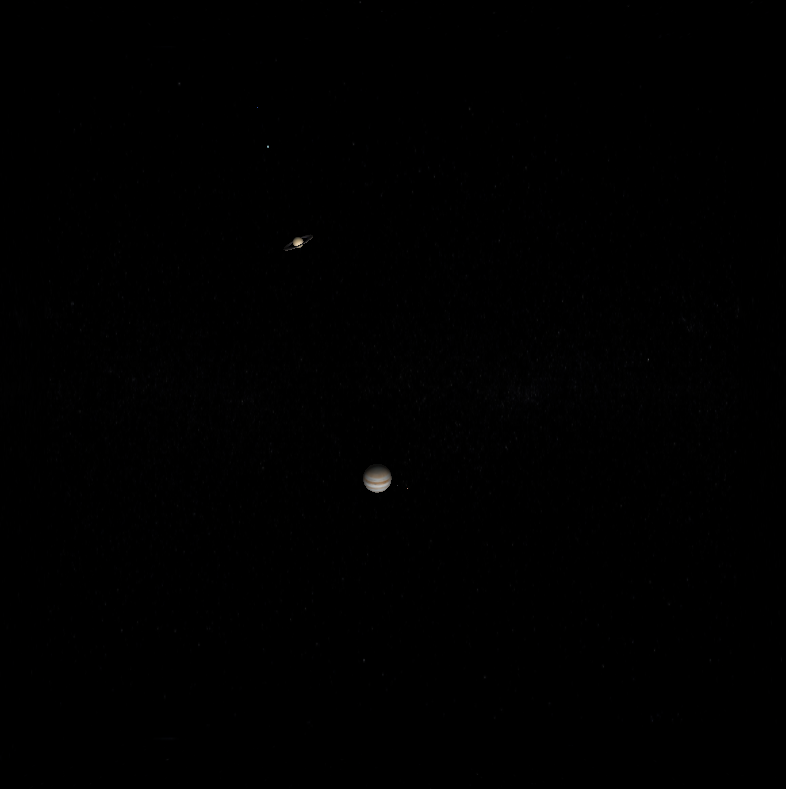
\includegraphics[width = 8cm,height = 8cm]{jupiter.png}
  \caption{\texttt{}}
  \label{fig:jupiter}
\end{subfigure}%
\begin{subfigure}{0.5\textwidth}
  \centering
  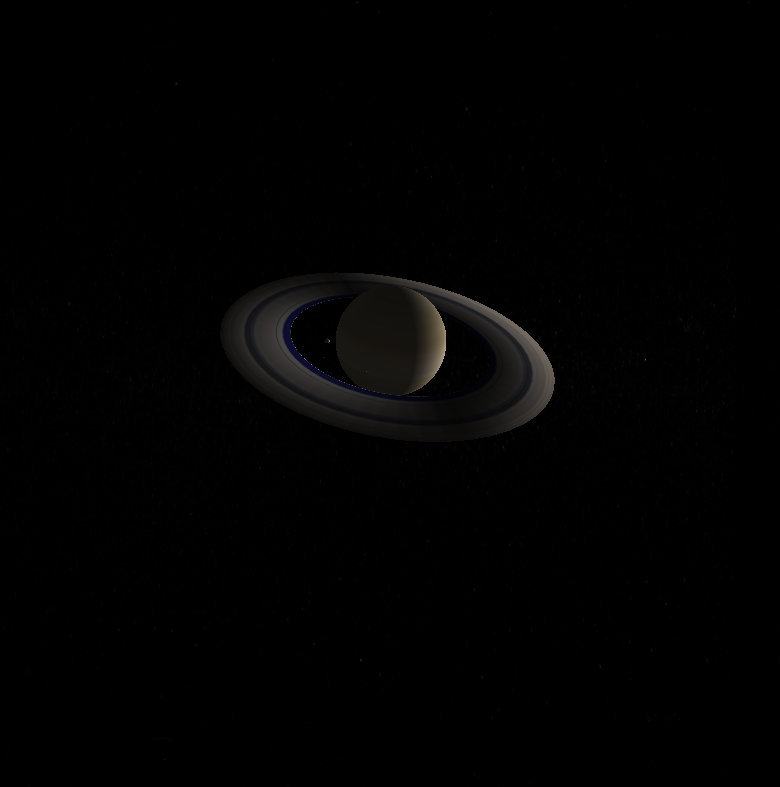
\includegraphics[width = 8cm,height = 8cm]{saturn.png}
  \caption{\texttt{}}
  \label{fig:saturn}
\end{subfigure}
\label{fig:texturas}
\caption{Texturas}
\end{figure}



\newpage
\section{Extras}
Como extra, alterou-se o \textit{engine} por forma a colocar uma textura de fundo.
Para tal, é desenhado um cubo invertido antes de colocar a câmara. O \textit{xml} passa também a ter o campo \textit{background} onde se define a textura de fundo da cena.

\subsection{Demonstração}

\vspace{1cm}
\begin{figure}[H]
\centering
\begin{subfigure}{0.5\textwidth}
  \centering
  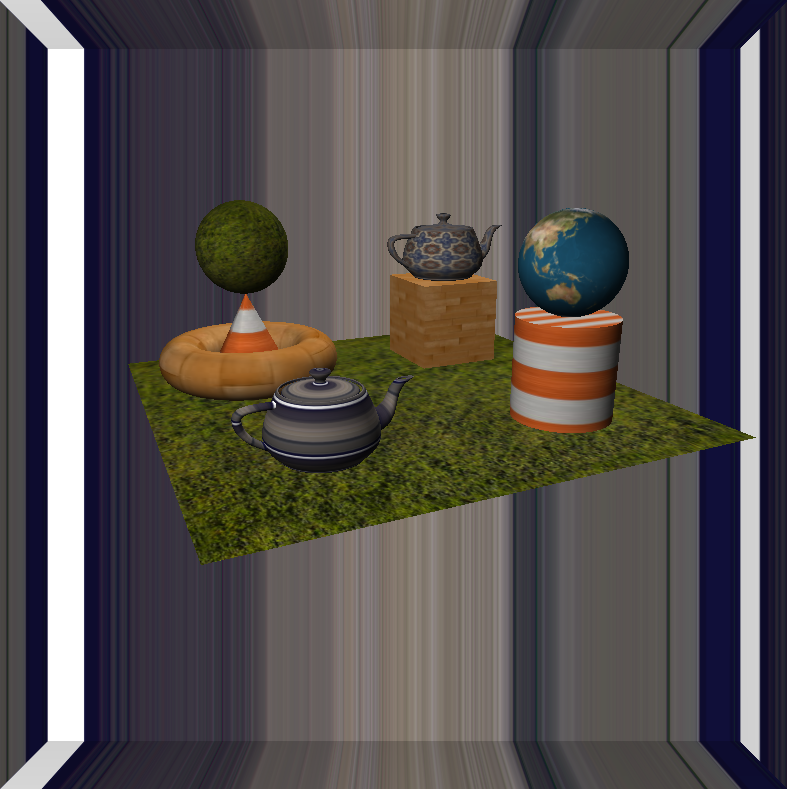
\includegraphics[width = 8cm,height = 8cm]{background_1.png}
  \caption{\texttt{}}
  \label{fig:background_1}
\end{subfigure}%
\begin{subfigure}{0.5\textwidth}
  \centering
  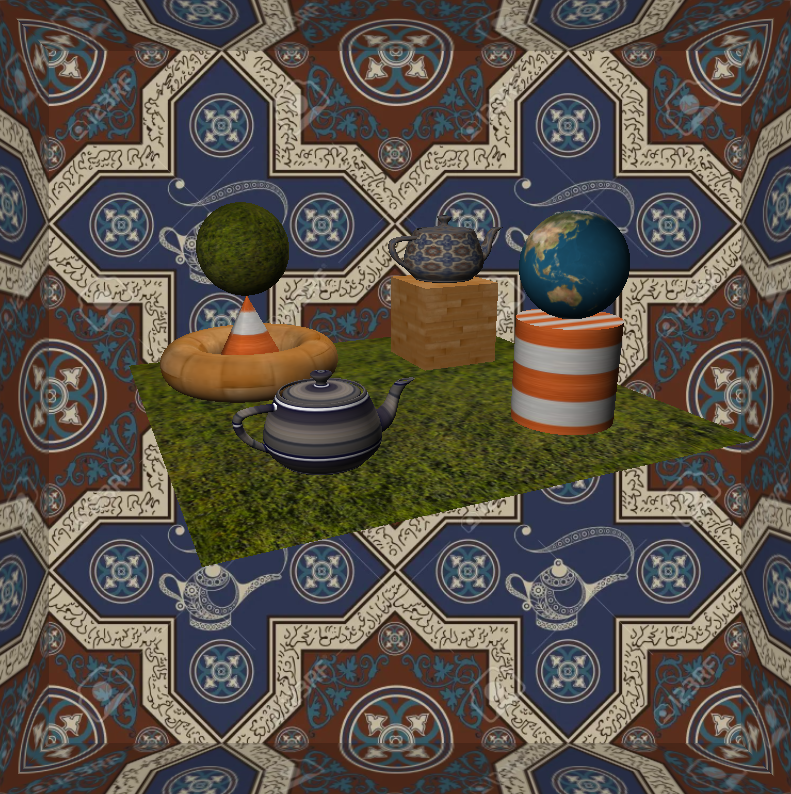
\includegraphics[width = 8cm,height = 8cm]{background_2.png}
  \caption{\texttt{}}
  \label{fig:background_2}
\end{subfigure}
\label{fig:texturas}
\caption{Textura de fundo}
\end{figure}




\newpage
\chapter{Conclusão}
Esta fase do projeto foi a que requereu mais alterações tanto no \texbf{engine} como no \texbf{generator}, no entanto, devido ás decisões tomadas nas fases anteriores que tornaram os dois programas escaláveis, essas alterações tornaram-se simples de fazer. 

A principal dificuldade foi encontrar as estratégias certas para o cálculo das normais e coordenadas de textura das primitivas.

O grupo considera que todos os objetivos propostos foram atingidos.

\end{document}
